% Solution to the Lecture 5 homework "Tacit collusion in oligopoly" (Aula/Lecture05.pdf, slide 34).
% Compile: pdflatex homework-lecture-05.tex (twice). Check: pdffonts (all Type 1, uni = yes).
% Every number is asserted by homework-lecture-05-check.py in this folder.
\documentclass[11pt,a4paper]{article}
\usepackage[utf8]{inputenc}
\usepackage[T1]{fontenc}
\usepackage{lmodern}   % Type 1 vector fonts (replaces PK bitmaps)
\usepackage{cmap}      % ToUnicode CMap -> copyable text and accents
\usepackage[english]{babel}
\usepackage{amsmath,amssymb,amsthm,mathtools}
\usepackage[a4paper,margin=2.4cm]{geometry}
\usepackage{microtype}
\usepackage{booktabs,array}
\usepackage{enumitem}
\usepackage{xcolor}
\usepackage{tikz}
\usetikzlibrary{arrows.meta,positioning,calc}
\usepackage[most]{tcolorbox}
\usepackage{fancyhdr}
\usepackage[hidelinks]{hyperref}

\setlist{topsep=3pt,itemsep=2pt}
\setlength{\parindent}{0pt}
\setlength{\parskip}{5pt}
\renewcommand{\arraystretch}{1.2}
\allowdisplaybreaks

\pagestyle{fancy}\fancyhf{}
\lhead{\footnotesize Economics of Organizations and Incentives --- MPE Insper}
\rhead{\footnotesize Lecture 5 homework: solution}
\cfoot{\footnotesize\thepage}
\renewcommand{\headrulewidth}{0.3pt}
\setlength{\headheight}{14pt}

\definecolor{ans}{RGB}{20,110,70}
\definecolor{src}{RGB}{30,80,150}
\definecolor{fa}{RGB}{190,60,40}
\newcommand{\answer}[1]{\begin{tcolorbox}[colback=ans!5,colframe=ans,boxrule=0.6pt,
  left=5pt,right=5pt,top=3pt,bottom=3pt]\textbf{Answer.} #1\end{tcolorbox}}

\title{\textbf{Homework, Lecture 5: Tacit Collusion in Oligopoly}\\[4pt]
  \large Solution --- Economics of Organizations and Incentives (MPE Insper)}
\date{November 2026}

\begin{document}
\maketitle
\thispagestyle{empty}

\section*{The problem}

\textbf{Source.} Lecture 5 slides, \texttt{Aula/Lecture05.pdf}, slide 34 (Homework: tacit
collusion); no answer given. Reproduced verbatim.

\begin{tcolorbox}[colback=src!4,colframe=src,boxrule=0.5pt]
Two firms play the Cournot game from Lecture 2 repeatedly, forever, with discount factor
$\delta$: inverse demand $P = 100 - q_1 - q_2$ and cost $C(q_i) = 10\,q_i$.
\begin{enumerate}[leftmargin=1.6em,itemsep=1pt]
\item Find the Cournot-Nash outputs and profits of the stage game. Find the cartel outcome, in which
each firm produces half of the monopoly output, and the profit of each firm.
\item Suppose the rival produces the cartel output. What is the best deviation, and the profit it yields?
\item Write the grim-trigger strategy: produce the cartel output as long as both firms have done so;
otherwise, produce the Cournot-Nash output forever. Use the one-stage deviation principle to find the
values of $\delta$ for which it is a subgame-perfect equilibrium.
\item Show that the threshold does not depend on the demand and cost parameters: redo item 3 with
$P = a - b(q_1 + q_2)$ and marginal cost $c < a$.
\item Which market features make tacit collusion easier? Relate them to item 3.
\end{enumerate}
\end{tcolorbox}

\textbf{Notation (Lecture 5).} A history $h$ is the list of past action profiles; $h = \varnothing$ at the
start. A strategy $s_i$ maps each history into a quantity. Payoffs are normalised,
$U_i(s) = (1-\delta)\sum_{t\ge1}\delta^{t-1}u_i(a^t(s))$ (slide 21), so a constant stream $k$ is worth
$k$. $s|_h$ is the continuation strategy at $h$. The one-stage deviation principle (slide 25): $s$ is
an SPE iff for every history $h$, player $i$ and action $a_i$,
\[
U_i(s|_h) \;\ge\; (1-\delta)\,u_i\bigl(a_i, s_{-i}(h)\bigr) + \delta\, U_i\bigl(s|_{(h,(a_i,s_{-i}(h)))}\bigr).
\]
The method is that of grim trigger in the prisoner's dilemma (slides 28--29), where it gives
$\delta \ge 1/4$: check the cooperative state, then the punishment state.

\section{Item 1: stage-game Nash and cartel outcomes}

Firm $i$ solves $\max_{q_i}\,(100 - q_i - q_j - 10)\,q_i$. The first-order condition
$90 - 2q_i - q_j = 0$ gives the best response
\[
BR_i(q_j) = \frac{90 - q_j}{2}.
\]
In the symmetric Nash equilibrium $q = (90 - q)/2$, so $q_N = 30$. Industry output is $60$, the price is
$40$, and each firm earns
\[
\pi_N = (40 - 10)\cdot 30 = 900.
\]
\emph{Cartel.} A monopolist maximises $(100 - Q - 10)Q$: $90 - 2Q = 0$, so $Q^m = 45$, the price is $55$
and the monopoly profit is $(55 - 10)\cdot 45 = 2025$. Each firm produces half, $q_C = 22.5$, and earns
\[
\pi_C = \frac{2025}{2} = 1012.5 \;>\; \pi_N = 900.
\]
\answer{Cournot-Nash: $q_N = 30$ each, price $40$, $\pi_N = 900$. Cartel: $q_C = 22.5$ each (total $45$),
price $55$, $\pi_C = 1012.5$.}

\section{Item 2: the best deviation}

If the rival produces $q_C = 22.5$, firm $i$ maximises its stage profit against it:
\[
q_D = BR(22.5) = \frac{90 - 22.5}{2} = 33.75.
\]
Industry output is $33.75 + 22.5 = 56.25$, the price is $43.75$ and
\[
\pi_D = (43.75 - 10)\cdot 33.75 = 33.75^2 = 1139.0625.
\]
The ranking $\pi_D > \pi_C > \pi_N$ ($1139.0625 > 1012.5 > 900$) is the prisoner's-dilemma structure of
the stage game: cartel output is not a stage-game Nash equilibrium, and each firm gains
$\pi_D - \pi_C = 126.5625$ by cheating once. Being punished costs $\pi_C - \pi_N = 112.5$ per period.

\answer{Best deviation $q_D = 33.75$, profit $\pi_D = 1139.0625$.}

\begin{figure}[ht]
\centering
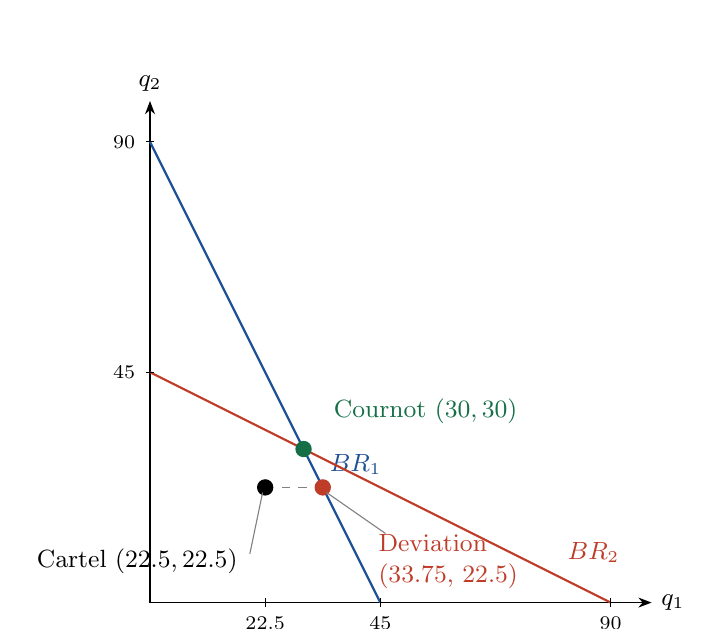
\begin{tikzpicture}[scale=0.065,>=Stealth,font=\small]
  \draw[->] (0,0) -- (98,0) node[right] {$q_1$};
  \draw[->] (0,0) -- (0,98) node[above] {$q_2$};
  \draw[thick,src] (45,0) -- (0,90) node[pos=0.3,right=3pt] {$BR_1$};
  \draw[thick,fa] (0,45) -- (90,0) node[pos=0.88,above right=1pt] {$BR_2$};
  \draw[dashed,gray] (22.5,22.5) -- (33.75,22.5);
  \fill[ans] (30,30) circle (1.6);
  \node[ans,anchor=south west] at (34,33) {Cournot $(30,30)$};
  \fill[black] (22.5,22.5) circle (1.6);
  \node[anchor=east] at (19,8) {Cartel $(22.5,22.5)$};
  \draw[gray] (19.5,9.5) -- (22,21.5);
  \fill[fa] (33.75,22.5) circle (1.6);
  \node[fa,anchor=west,align=left,inner sep=1pt] at (44,8) {Deviation\\$(33.75,\,22.5)$};
  \draw[gray] (46,13.5) -- (34.5,21.5);
  \foreach \x in {22.5,45,90} {\draw (\x,0.8) -- (\x,-0.8);}
  \foreach \y in {45,90} {\draw (0.8,\y) -- (-0.8,\y);}
  \node[below] at (22.5,-1) {\scriptsize 22.5};
  \node[below] at (45,-1) {\scriptsize 45};
  \node[below] at (90,-1) {\scriptsize 90};
  \node[left] at (-1,45) {\scriptsize 45};
  \node[left] at (-1,90) {\scriptsize 90};
\end{tikzpicture}
\caption{Best-response functions. The deviation point lies on firm 1's best response to the cartel
output $q_2 = 22.5$. Payoffs $(\pi_1, \pi_2)$: cartel $(1012.5,\ 1012.5)$, deviation $(1139.0625,\ 759.375)$,
Cournot $(900,\ 900)$.}
\end{figure}

\section{Item 3: grim trigger and the one-stage deviation principle}

\textbf{Strategy.} Let $h^t_C$ denote a history in which both firms produced $q_C$ in every past period
(and $h = \varnothing$). For firm $i$,
\[
s_i(h) = \begin{cases} 22.5 & \text{if } h = \varnothing \text{ or } h = h^t_C,\\ 30 & \text{otherwise.}\end{cases}
\]
There are two states, as in slide 28: \emph{collusion} (both have always produced $q_C$) and
\emph{punishment} (anyone ever deviated; absorbing, so cartel output never resumes).

\textbf{Collusion state.} Following $s$ gives $\pi_C$ forever, so $U_i(s|_h) = \pi_C$ (normalised).
The best one-stage deviation is $q_D$, which yields $\pi_D$ today and moves play to the punishment state,
worth $\pi_N$ per period. The constraint is
\[
\pi_C \;\ge\; (1-\delta)\,\pi_D + \delta\,\pi_N.
\]
Equivalently, in unnormalised form, $\dfrac{\pi_C}{1-\delta} \ge \pi_D + \dfrac{\delta\,\pi_N}{1-\delta}$.
Rearranging, $(1-\delta)(\pi_D - \pi_C) \le \delta\,(\pi_C - \pi_N)$, so
\[
\delta \;\ge\; \delta^* = \frac{\pi_D - \pi_C}{\pi_D - \pi_N} = \frac{126.5625}{239.0625} = \frac{9}{17} \approx 0.529.
\]
(Here $\pi_D - \pi_N = 1139.0625 - 900 = 239.0625$.) The numerator is the one-period gain from cheating;
the denominator is that gain plus the per-period loss from punishment. So $\delta^*$ is the share of the
total at stake that the future must outweigh. At $\delta = 1/2$: $\pi_C = 1012.5$ against
$\tfrac12\cdot 1139.0625 + \tfrac12\cdot 900 = 1019.53125$, so cheating pays. At $\delta = 0.6$
cooperation wins.

\textbf{Punishment state (off the path).} After any history other than $h^t_C$, $s$ prescribes $q_N = 30$
forever; the continuation payoff is $\pi_N = 900$. A one-stage deviation to $x$ against a rival who plays
$30$ gives $(1-\delta)(100 - x - 30 - 10)x + \delta\cdot 900$, and the stage profit $(60 - x)x$ is maximised
at $x = 30$, where it equals $900$. So no one-shot deviation is profitable, for any $\delta$: the
Cournot-Nash profile is a Nash equilibrium of the stage game, and playing it after any history is
credible. This is the argument of slide 29 (``which always holds: $(F,f)$ is a Nash equilibrium of
the stage game'').

\textbf{Conclusion.} The only binding constraint is the collusion state. By the one-stage deviation
principle, grim trigger is a subgame-perfect equilibrium iff $\delta \ge 9/17$. For $\delta < 9/17$
the cartel output is not sustainable by this punishment.

\answer{Grim trigger is an SPE iff $\delta \ge \delta^* = 9/17 \approx 0.529$.}

\begin{figure}[ht]
\centering
\begin{tikzpicture}[scale=1,>=Stealth,font=\small]
  \draw[->] (0,0) -- (8.2,0) node[right] {period $t$};
  \draw[->] (0,0) -- (0,4.2) node[above] {stage profit};
  \draw[thick,ans] (0,2.8125) -- (8,2.8125) node[right] {\scriptsize comply: $1012.5$};
  \draw[thick,fa] (0,3.16) -- (1,3.16);
  \draw[thick,fa] (1,2.5) -- (8,2.5) node[right] {\scriptsize deviate, then punished: $900$};
  \node[fa,above] at (0.5,3.16) {\scriptsize $1139.0625$};
  \draw[dotted] (0,2.5) -- (1,2.5);
  \node[left] at (0,2.5) {\scriptsize 900};
  \node[left] at (0,2.8125) {\scriptsize 1012.5};
  \foreach \x/\l in {0.5/1,1.5/2,2.5/3} {\node[below] at (\x,0) {\scriptsize \l};}
\end{tikzpicture}
\caption{Stage profits under compliance and after a deviation in period 1 (vertical axis not to scale from
zero). The deviator gains $126.5625$ once and loses $112.5$ in every later period; discounting decides
which dominates, and the break-even is $\delta^* = 9/17$.}
\end{figure}

\section{Item 4: general demand and cost}

Let $P = a - bQ$ with $b > 0$ and marginal cost $c < a$, and write $k = (a-c)^2/b$.
\begin{itemize}
\item \emph{Best response:} $\max_{q_i}(a - b(q_i + q_j) - c)q_i$ gives $BR(q_j) = \dfrac{a - c - b\,q_j}{2b}$.
\item \emph{Cournot:} $q = BR(q)$ gives $q_N = \dfrac{a-c}{3b}$ and
$\pi_N = \dfrac{(a-c)^2}{9b} = \dfrac{k}{9}$.
\item \emph{Cartel:} $Q^m = \dfrac{a-c}{2b}$, so $q_C = \dfrac{a-c}{4b}$ and
$\pi_C = \dfrac{(a-c)^2}{8b} = \dfrac{k}{8}$ (half of the monopoly profit $k/4$).
\item \emph{Deviation:} $q_D = BR(q_C) = \dfrac{3(a-c)}{8b}$. The margin is $a - b(q_D + q_C) - c =
\dfrac{3(a-c)}{8}$, so $\pi_D = \dfrac{9(a-c)^2}{64\,b} = \dfrac{9k}{64}$.
\end{itemize}
Every profit is proportional to the single scale factor $k$. Hence
\[
\pi_D - \pi_C = \Bigl(\tfrac{9}{64} - \tfrac{8}{64}\Bigr)k = \frac{k}{64}, \qquad
\pi_D - \pi_N = \Bigl(\tfrac{9}{64} - \tfrac{1}{9}\Bigr)k = \frac{17\,k}{576},
\]
\[
\delta^* = \frac{\pi_D - \pi_C}{\pi_D - \pi_N} = \frac{k/64}{17k/576} = \frac{576}{64\cdot17} = \frac{9}{17}.
\]
The off-path check is unchanged: Cournot-Nash is a stage-game equilibrium whatever $(a, b, c)$. The
parameters only rescale the profit units, and the threshold is a ratio of profit differences, so the scale
cancels. With $a = 100$, $b = 1$, $c = 10$: $k = 8100$ and the profits are $900$, $1012.5$, $1139.0625$, as
in items 1--2. What does matter is the \emph{structure} (linear demand, constant marginal cost, two
symmetric firms, Cournot punishment); the next item changes it.

\answer{$\pi_N = (a-c)^2/9b$, $\pi_C = (a-c)^2/8b$, $\pi_D = 9(a-c)^2/64b$, and $\delta^* = 9/17$ for every
$b > 0$ and $c < a$.}

\section{Item 5: what makes tacit collusion easier}

Item 3 says collusion is sustainable iff
\[
\underbrace{(1-\delta)}_{\text{weight on today}}\underbrace{(\pi_D - \pi_C)}_{\text{gain from cheating}}
\;\le\; \underbrace{\delta}_{\text{weight on tomorrow}}\underbrace{(\pi_C - \pi_N)}_{\text{loss per period}} .
\]
Anything that raises $\delta$, lowers the gain from cheating, or raises the loss from punishment helps.

\textbf{1. Few firms.} With $n$ symmetric firms, the Cournot output is $q_N = (a-c)/((n+1)b)$ and
$\pi_N = k/(n+1)^2$. The cartel shares the monopoly profit, so $\pi_C = k/(4n)$. The deviator best-responds
to $n-1$ rivals each producing $(a-c)/(2nb)$, so $q_D = (n+1)(a-c)/(4nb)$ and
$\pi_D = k(n+1)^2/(16n^2)$. Then the gain is $\pi_D - \pi_C = k(n-1)^2/(16n^2)$, the loss is
$\pi_C - \pi_N = k(n-1)^2/(4n(n+1)^2)$, and
\[
\frac{\text{gain}}{\text{loss}} = \frac{(n+1)^2}{4n}, \qquad
\delta^*(n) = \frac{\pi_D - \pi_C}{\pi_D - \pi_N} = \frac{(n+1)^2}{n^2 + 6n + 1}.
\]
\begin{center}
\begin{tabular}{c|ccccccccc}
$n$ & 2 & 3 & 4 & 5 & 6 & 7 & 8 & 9 & 10\\\hline
$\delta^*$ & $\frac{9}{17}$ & $\frac{4}{7}$ & $\frac{25}{41}$ & $\frac{9}{14}$ & $\frac{49}{73}$ &
$\frac{16}{23}$ & $\frac{81}{113}$ & $\frac{25}{34}$ & $\frac{121}{161}$\\
$\approx$ & 0.529 & 0.571 & 0.610 & 0.643 & 0.671 & 0.696 & 0.717 & 0.735 & 0.752
\end{tabular}
\end{center}
$\delta^*(n)$ is increasing in $n$ and tends to $1$. In the inequality: the ratio gain/loss grows with
$n$, because the punishment loss $\pi_C - \pi_N$ shrinks fast (Cournot with many firms is already close
to competitive) while the temptation to undercut a cartel that restrains output stays large. Concentration
and entry barriers facilitate collusion; entry or a competitive fringe breaks it.

\textbf{2. Frequent interaction.} Write $\delta = e^{-r\Delta t}$, where $r$ is the interest rate and
$\Delta t$ the time between decisions. The duopoly condition $\delta \ge 9/17$ is
$r\Delta t \le \ln(17/9) \approx 0.636$. Shorter periods (frequent, repeated sales), a low interest rate
and a high probability that the market continues (slide 22: $\delta$ also reflects the chance the
relationship ends) all raise $\delta$. Infrequent, lumpy sales (one-off auctions, long gaps between
orders) are hard to collude in.

\textbf{3. Observability and speed of detection.} The strategy needs each firm to see the deviation
and to retaliate. If detection takes several periods, the deviator enjoys $\pi_D$ for all of them, so
the effective gain from cheating in item 3 rises. Posted prices and public sales data shorten the lag;
secret discounts and hidden quantities lengthen it. With imperfect monitoring (Green--Porter), a low price may
reflect a demand shock rather than cheating, so firms must punish on bad signals and price wars occur
on the equilibrium path; this lowers the value of collusion below $\pi_C$ forever.

\textbf{4. Demand growth or decline.} Growing demand raises the profit stakes of later periods, which acts
like a higher $\delta$: the future loss from punishment is larger relative to today's gain, so collusion is
easier. Declining demand, or a market near its end, does the opposite; a known last period makes
cooperation unravel (Lecture 5, finitely repeated games). Temporary demand booms raise today's
gain $\pi_D - \pi_C$ relative to the future, so collusion is most fragile in booms.

\textbf{5. Symmetry.} Item 3 assumed identical firms. When firms differ in costs, capacity or
patience, each has its own threshold and the cartel needs all of them satisfied; the firm with the largest
deviation gain or the lowest $\delta$ binds. Similar costs, products and shares make a common cartel
output and punishment natural.

\textbf{6. Multimarket contact.} If the same firms meet in several markets, a deviation in one can be
punished in all, so the loss in the right-hand side of the inequality is larger. Slack in one market's
constraint also supports a market where the constraint binds.

\textbf{7. Capacity.} Spare capacity in the hands of rivals makes punishment credible and costly (a
larger loss), but spare capacity in the hands of a potential cheater makes cheating cheap and large (a
larger gain). Collusion is easiest when capacity is similar and roughly matched to the cartel output.

\textbf{Remark: softer punishment.} Nash reversion is not the harshest credible punishment. Abreu's
carrot-and-stick strategies (a short, severe punishment phase, then a return to collusion) can drive the
punishment payoff below $\pi_N$ for a while, which lowers the threshold below $9/17$ for the same cartel
output. I give no number for this; the script does not verify one.

\section*{References}
\begin{itemize}[leftmargin=1.4em]
\item Lecture 5 slides (\texttt{Aula/Lecture05.pdf}): slide 21 (normalised payoffs), slide 22 (interpreting
discounting), slide 25 (one-stage deviation principle), slides 28--29 (grim trigger), slide 34 (this homework).
\item Tadelis, S. (2013), \emph{Game Theory: An Introduction}, Princeton University Press,
Section 10.4 ``Application: Tacit Collusion'', p.~201 (the same Cournot example).
\item Cabral, L. (2017), \emph{Introduction to Industrial Organization}, 2nd ed., MIT Press, Chapter 9
``Collusion and Price Wars'', Section 9.3 ``Factors that facilitate collusion'', p.~227.
\item Gibbons, R. (1992), \emph{Game Theory for Applied Economists}, Princeton University Press,
Section 2.3.C ``Collusion between Cournot Duopolists'', p.~102.
\item Green, E. and Porter, R. (1984), ``Noncooperative collusion under imperfect price information'',
\emph{Econometrica} 52(1); Abreu, D. (1986), ``Extremal equilibria of oligopolistic supergames'',
\emph{Journal of Economic Theory} 39(1): cited from memory, without pages.
\end{itemize}

\end{document}
